\documentclass{TIJMUjiaoanLL}
\pagestyle{empty}


\begin{document}


%课程名称
\kecheng{系统生物学}
%课程内容
\neirong{基因组学(测序数据分析)\ /\ 第2章}
%教师姓名
\jiaoshi{伊现富}
%职称
\zhicheng{讲师}
%教学日期(格式:XXXX年XX月XX日XX时-XX时)
\riqi{2016年9月20日13:30-15:30}
%授课对象(格式:XXX系XXXX年级XX班(硕/本/专科))
\duixiang{生物医学工程与技术学院2013级生信班(本)}
%听课人数
\renshu{28}
%授课方式
\fangshi{理论讲授}
%学时数
\xueshi{2}
%教材版本
\jiaocai{系统生物学,第1版}


%教案首页
\firstHeader
\maketitle
\thispagestyle{empty}

\mudi{
\begin{itemize}
  \item 掌握FASTQ、BED、GFF等数据格式,第二代测序数据分析的基本流程,外显子组测序的分析步骤。
  \item 熟悉SAM、VCF等数据格式,测序深度、覆盖度等术语,测序数据分析的常用工具。
  \item 了解SRA、GEO等数据库,外显子组测序的流程和应用。
  \item 自学SRA、GEO等数据库的使用,测序数据分析常用工具的使用。
\end{itemize}
}

\fenpei{
\begin{itemize}
  \item (5')引言与导入:回顾第二代测序的主要技术和基本流程。
  \item (30')数据库与数据格式:介绍SRA和GEO等与第二代测序相关的数据库,讲解第二代测序数据分析中常见的FASTQ、SAM、BED、GFF和VCF等数据格式。
  \item (40')测序数据分析:讲解测序深度和覆盖度等术语,总结测序数据分析的主要流程,介绍分析流程中每个步骤的作用、常用工具和注意事项。
  \item (20')外显子组测序:介绍外显子组测序的基本流程,讲解外显子组测序数据分析的基本步骤,通过实例介绍外显子组测序的应用。
  \item (5')总结与答疑:总结授课内容中的知识点与技能,解答学生疑问。
\end{itemize}
}

\zhongdian{
\begin{itemize}
  \item 重点:FASTQ、BED、GFF等数据格式,第二代测序数据的分析流程。
  \item 难点:SAM、VCF等数据格式。
  \item 解决策略:通过实例讲解和比较类比帮助学生理解、记忆。
\end{itemize}
}

\waiyu{
  \vspace*{-10pt}
  \begin{multicols}{2}
    深度(depth)

    覆盖度(coverage)

    质量控制(QC,quality control)

    预处理(preprocessing)

    外显子组测序(WES,whole exome sequencing)

    全基因组测序(WGS,whole genome sequencing)
  \end{multicols}
  \vspace*{-10pt}
}

\fuzhu{
\begin{itemize}
  \item 多媒体:与第二代测序相关的数据库和数据格式。
  \item 板书:第二代测序数据的分析流程。
\end{itemize}
}

\sikao{
  \vspace*{-10pt}
  \begin{multicols}{2}
  \begin{itemize}
    \item 举例说明FASTQ、BED和GFF数据格式。
    \item 解释测序深度和覆盖度。
    \item 总结测序数据分析的基本流程。
    \item 列举测序数据分析中的常用工具。
  \end{itemize}
  \end{multicols}
  \vspace*{-10pt}
}

\cankao{
\begin{itemize}
  \item 维基百科等网络资源。
\end{itemize}
}

\firstTail


%教案续页
\newpage
\otherHeader

\begin{enumerate}
  \item 引言与导入(5分钟)
    \begin{enumerate}
      \item 测序历史:第一代(Sanger) $\Rightarrow$ 第二代(高通量) $\Rightarrow$ 第三代(单分子)
      \item 二代测序:Roche/454,Illumina/Solexa(桥式扩增+边合成边测序),ABI/SOLiD
    \end{enumerate}

  \item 数据库与数据格式(30分钟)
    \begin{enumerate}
      \item 数据库
        \begin{itemize}
          \item 测序数据:SRA(Sequence Read Archive),GEO(Gene Expression Omnibus)
          \item 肿瘤相关:TCGA(Cancer Genome Atlas),ICGC(International Cancer Consortium)
          \item 其他:1000 Genomes Project
        \end{itemize}
      \item 数据格式
        \begin{enumerate}
\parpic[fr]{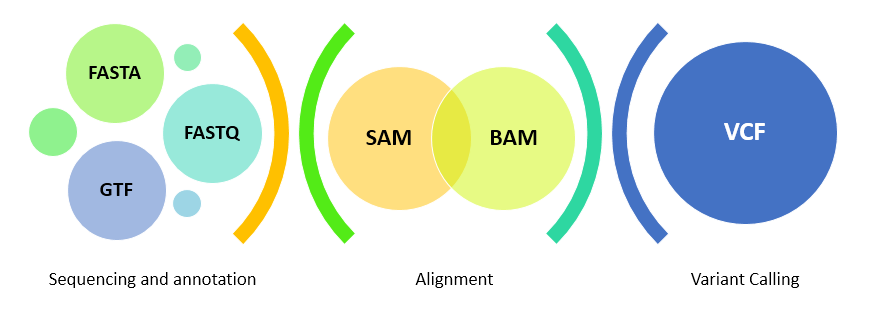
\includegraphics[width=8cm]{c2.format.list.02.png}}
          \item 简介
            \begin{itemize}
              \item 序列与读段:FASTA、2bit,FASTQ
              \item 读段比对:SAM、BAM
              \item 特征注释:BED、GTF/GFF
              \item 变异信息:VCF、BCF
            \end{itemize}
          \item 序列格式:FASTA和FASTQ
            \vspace{-0.5em}
            \begin{figure}[h]
              \centering
              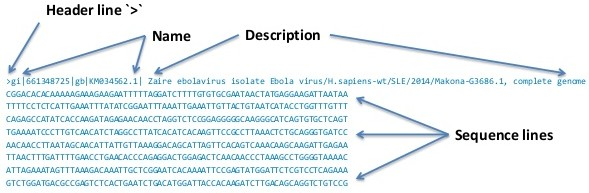
\includegraphics[width=0.45\textwidth]{c2.format.fasta.01.jpg}
              \quad
              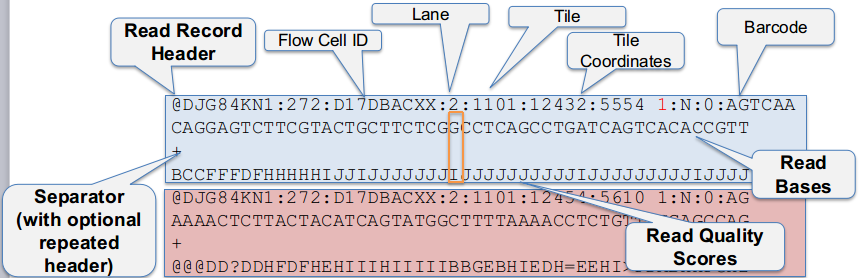
\includegraphics[width=0.45\textwidth]{c2.format.fastq.01.png}
            \end{figure}
            \begin{itemize}
            \vspace{-0.5em}
\parpic[fr]{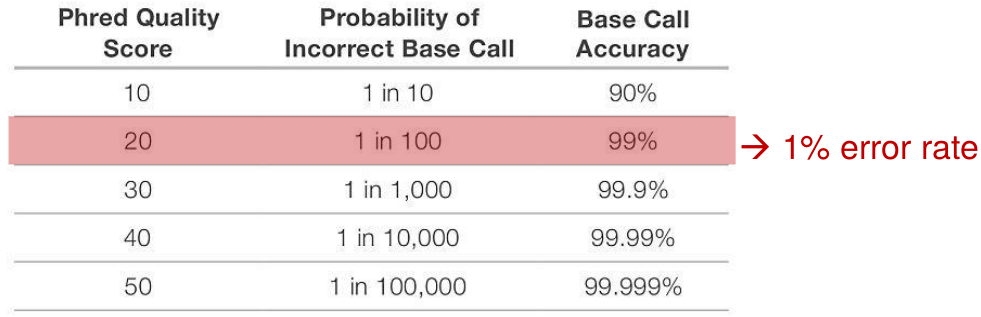
\includegraphics[width=8cm]{c2.format.fastq.qual.06.png}}
              \item FASTQ = FASTA + PHRED (quality score)
              \item 常用后缀:.fq, .fastq
              \item ID:/1和/2$\Rightarrow$PE
              \item PHRED:$Q_{sanger} = -10log_{10}p$
            \vspace{-0.5em}
            \begin{figure}[h]
              \centering
              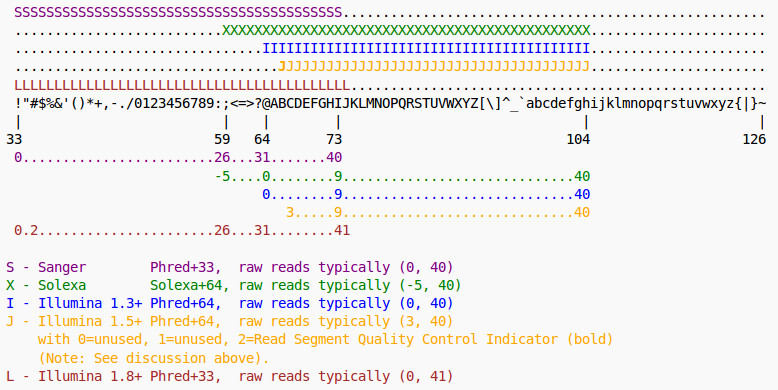
\includegraphics[width=0.4\textwidth]{c2.format.fastq.qual.04.png}
              \quad
              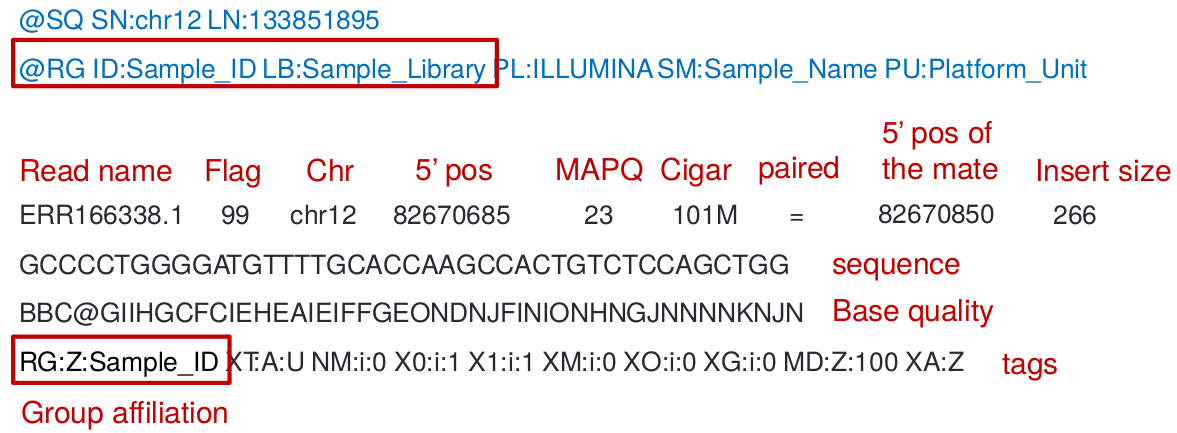
\includegraphics[width=0.55\textwidth]{c2.format.sam.32.png}
            \end{figure}
            \vspace{-0.5em}
            \end{itemize}
          \item 比对格式:SAM
            \begin{itemize}
              \item SAM:Sequence Alignment/Map format, human readable
              \item BAM:Binary version of SAM, compress$\Rightarrow$smaller, index$\Rightarrow$random access
            \end{itemize}
          \item 注释格式:BED和GTF/GFF
            \begin{itemize}
\parpic[fr]{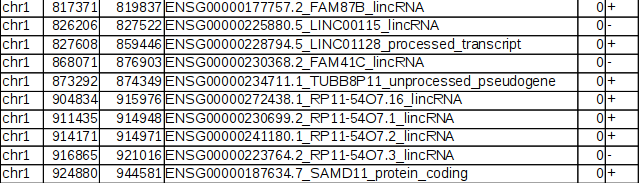
\includegraphics[width=8cm]{c2.format.bed.10.png}}
              \item BED$\Rightarrow$bigBed, bedGraph
              \item GTF: GFF2.5, Gene Transfer Format
              \item GFF: GFF3, General Feature Format
              \item 坐标系统
                \begin{itemize}
                  \item BED: [0-based), length=stop-start
                  \item GTF/GFF: [1-based], lengt=stop-start+1
                \end{itemize}
            \end{itemize}

\otherTail
\newpage
\otherHeader

          \item 变异格式:VCF
            \vspace{-0.5em}
            \begin{figure}[h]
              \centering
              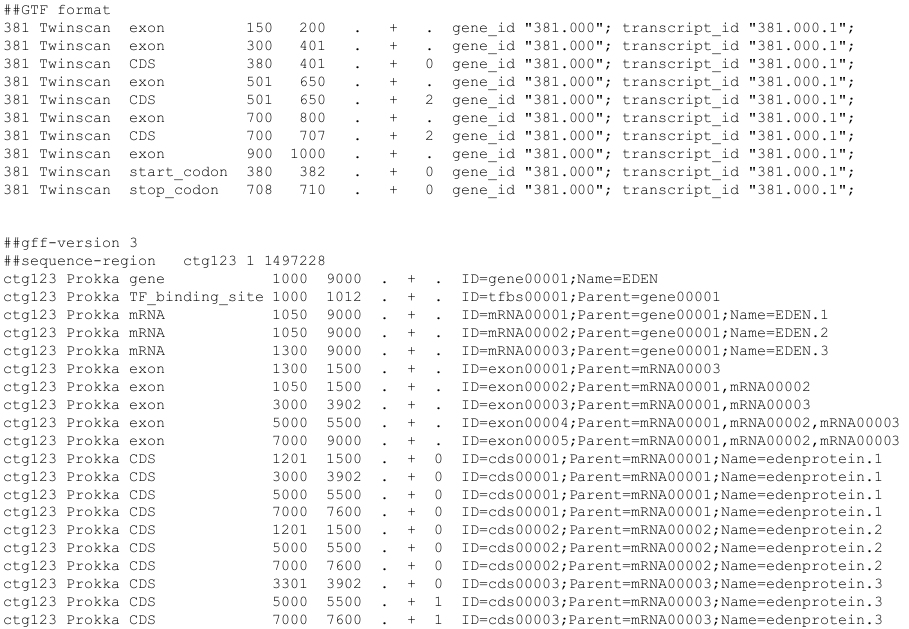
\includegraphics[width=0.5\textwidth]{c2.format.gtf.gff.03.png}
              \quad
              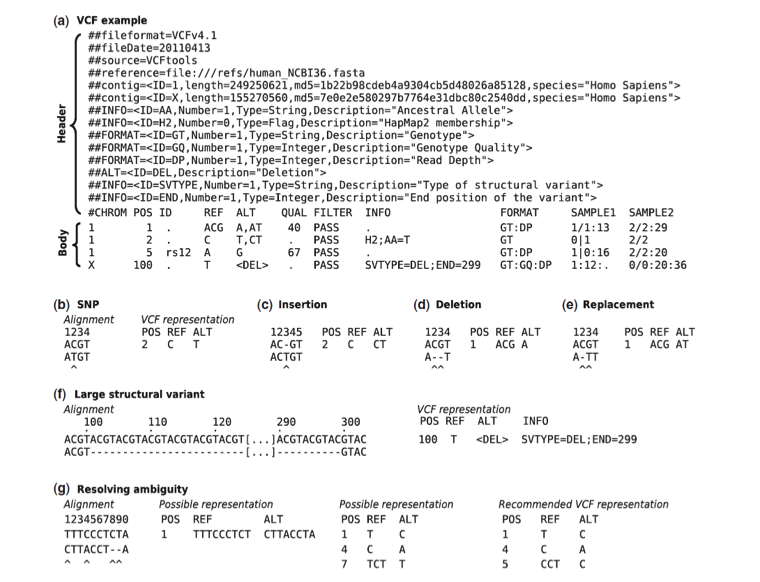
\includegraphics[width=0.45\textwidth]{c2.format.vcf.06.png}
            \end{figure}
            \vspace{-0.5em}
        \end{enumerate}
    \end{enumerate}

\parpic[fr]{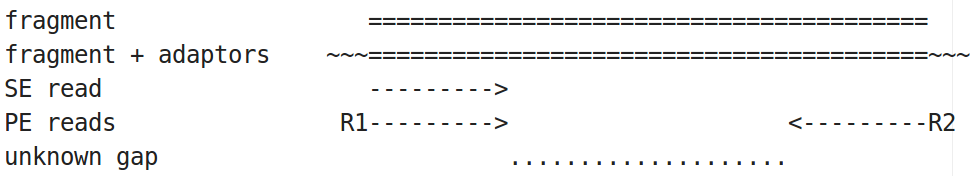
\includegraphics[width=8cm]{c2.term.insert.size.01.png}}
  \item 测序数据分析(40分钟)
    \begin{enumerate}
      \item 常见术语
        \begin{itemize}
          \item 深度:测序得到的总碱基数与待测基因组大小的比值
          \item 覆盖度:测序获得的序列占整个基因组的比例
\parpic[fr]{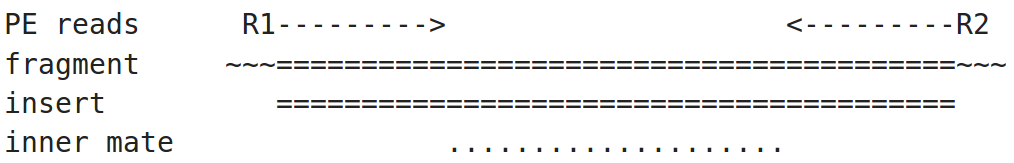
\includegraphics[width=8cm]{c2.term.insert.size.02.png}}
          \item SE(single end) vs.PE(paired end)
          \item PE: insert vs. inner mate distance
        \end{itemize}
      \item 分析流程
            \vspace{-0.5em}
            \begin{figure}[h]
              \centering
              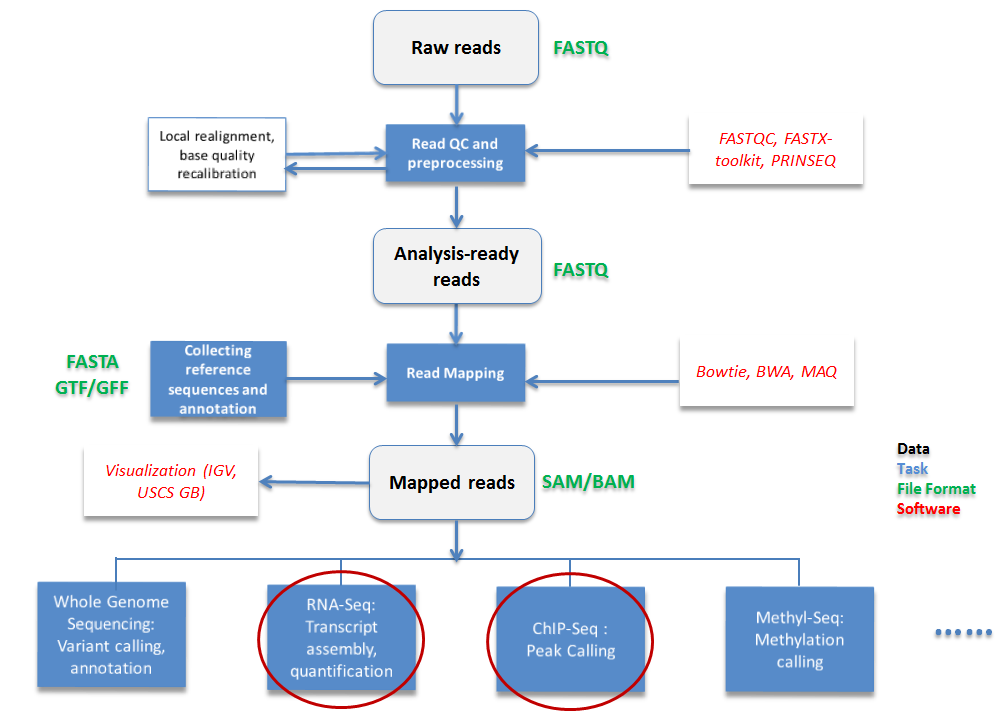
\includegraphics[width=0.4\textwidth]{c2.workflow.ngs.03.png}
              \quad
              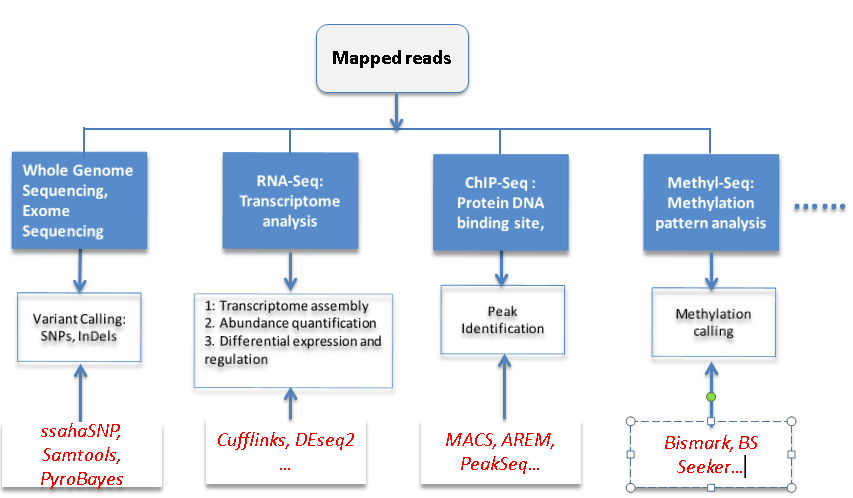
\includegraphics[width=0.5\textwidth]{c2.workflow.ngs.04.png}
            \end{figure}
            \vspace{-0.5em}
            \begin{enumerate}
              \item Quality Control: FastQC, NGS QC Toolkit, SolexaQA
              \item Preprocessing(trim \& filter): FASTX-Toolkit, PRINSEQ
              \item Mapping: BWA, Bowtie, SOAP
\parpic[fr]{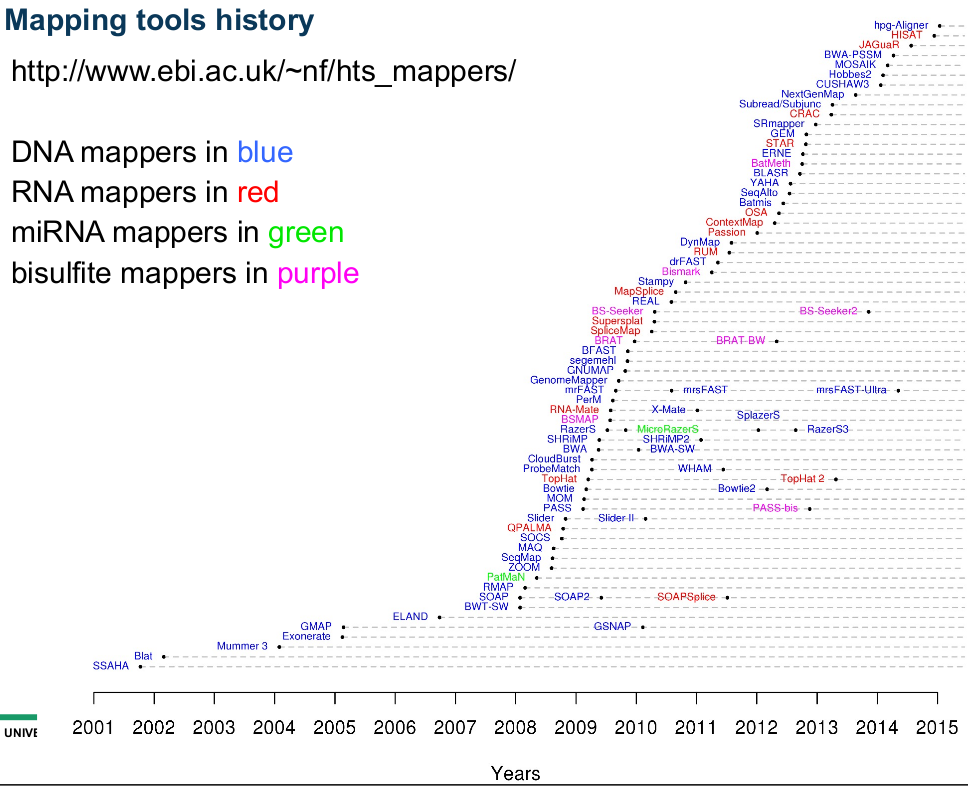
\includegraphics[width=7.5cm]{c2.tool.alignment.04.png}}
              \item Calling Variants: Samtools, GATK, VarScan
              \item Variant Annotation: SnpEff, ANNOVAR, SeattleSeq Annotation, SIFT, PolyPhen-2
              \item Visualization: Genome Browser, IGV, Tablet, Circos
              \item Others: Galaxy, Picard, bedtools, BEDOPS, csvkit
            \end{enumerate}
      \item 补遗
        \begin{itemize}
          \item Removal of PCR duplicates
          \item Indel Realignment
          \item Base quality recalibration
          \item Ohters: Replicates(biological vs. technical), depth, length, SE vs. PE
        \end{itemize}
    \end{enumerate}

\otherTail
\newpage
\otherHeader

  \item 外显子组测序(20分钟)
    \begin{enumerate}
\parpic[fr]{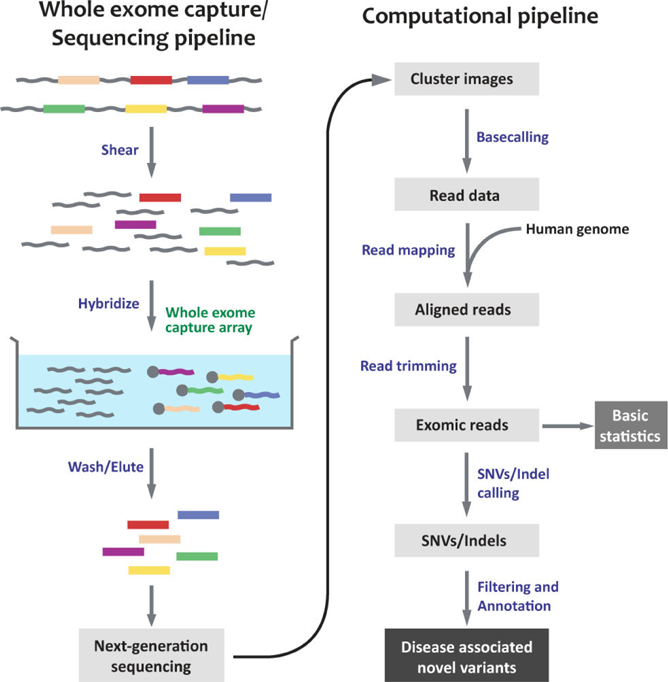
\includegraphics[width=9.5cm]{c2.exome.exp.bx.01.jpg}}
      \item 基本概念
        \begin{itemize}
          \item exome:genome $\Rightarrow$ 1\%,30Mb
          \item WES:exome $\Rightarrow$ sequencing
          \item WGS:genome $\Rightarrow$ sequencing
        \end{itemize}
      \item \textcolor{red}{【重点】}流程:实验 + 分析
      \item 应用实例
    \end{enumerate}

  \item 总结与答疑(5分钟)
    \begin{enumerate}
      \item 知识点
	\begin{itemize}
	  \item 数据库:SRA、GEO
    \item 数据格式:FASTQ、BED、GTF/GFF,\\ SAM、VCF
	  \item 测序术语:深度、覆盖度、PE
    \item 分析流程:QC、preprocessing, \\ mapping、variants、annotation, \\ visualization
	  \item 外显子组测序:实验与分析流程
	\end{itemize}
      \item 技能
	\begin{itemize}
    \item 测序数据分析软件:使用方法
	  \item 全基因组测序:数据分析
	  \item 外显子组测序:数据分析
	\end{itemize}
    \end{enumerate}
\end{enumerate}

\otherTail


\end{document}

